
\documentclass[titlepage]{article}
 \usepackage[utf8]{inputenc}
\usepackage{listings}
\usepackage{hyperref}
\usepackage{float}
\usepackage{graphicx}
\usepackage{subfig}
\graphicspath{ {imagenes/} }
 \usepackage{xcolor}
 \definecolor{RoyalBlue}{cmyk}{1, 0.50, 0, 0}

\lstset{language=Java,
	keywordstyle=\color{RoyalBlue},
	basicstyle=\scriptsize\ttfamily,
	commentstyle=\ttfamily\itshape\color{gray},
	stringstyle=\ttfamily,
	showstringspaces=false,
	breaklines=true,
	frameround=ffff,
	frame=single,
	rulecolor=\color{black}}


 

% Datos de la portada
\begin{document}
	

	\section{Random forest(RF)}	
	Se usa esta técnica puesto que es un muy buen clasificador. En este caso al meter información extra a el dataset tendremos una cantidad grande de variables y esta técnica trabaja muy bien cuando se tienen gran numero de variables. En este caso se ha añadido información de grado 2.
	\subsection{Especificación de parámetros RF} 
	En este caso nos hemos centrado en la elección de una buena cantidad de arboles y la cantidad de variables que utilizara cada árbol para predecir. Para seleccionar estos parámetros se han realizado varias pruebas con la partición de validación. Se ha medido el error con la partición de validación con tres cantidades distintas de variables. El numero de variables elegidas para cada una son las siguientes:
	\begin{enumerate}
		\item Raíz: En este caso se tendrá una cantidad de características para cada árbol igual a la raíz cuadrada del numero de características. 
		\item Mitad: La cantidad de variables sera en esta opción la mitad de las características.
		\item Cantidad de características: Para esta opción cada árbol utilizara todas las características.
	\end{enumerate}

	El numero de arboles lo iremos aumentando de 10 en 10 hasta llegar a 250. 
	
	Pasamos a mostrar el grafico para analizar el mejor numero de características para utilizar.
	\begin{figure}[H]
		\centering
		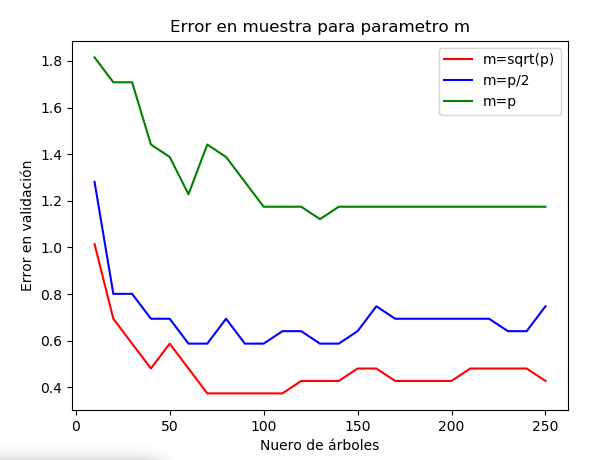
\includegraphics[width=0.7\linewidth]{../imagenesRF/errorvalidacion}
		\caption{}
		\label{fig:Cantidad de variables RF}
	\end{figure}
	En el grafico se ve claramente que la mejor opción es la raíz. También podemos sacar de este grafico cual es la mejor opción para el numero de arboles necesarios. En este caso a partir de 70 se tiende a igualar y no mejora. Para decidirnos por el numero de arboles tendremos en cuenta también el siguiente grafico, donde se muestra el tiempo de ejecución para cada cantidad de arboles.
	
	\begin{figure}[H]
		\centering
		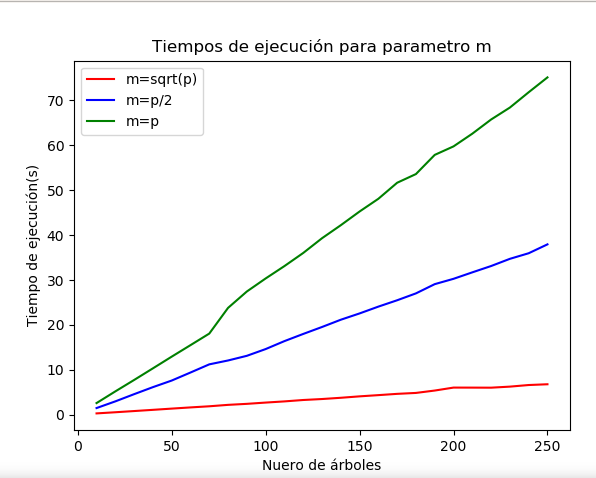
\includegraphics[width=0.7\linewidth]{../imagenesRF/tiempoEjecucion}
		\caption{}
		\label{fig:Tiempo de ejecucion}
	\end{figure}

	En este caso se ve que con mas cantidad de arboles tendremos una mayor tiempo de ejecución. Por tanto he decido definir la cantidad de arboles a 100 y quedarme con la opción de la raíz para el numero de características por árbol.
	
	
	\subsection{Valoracion de resultados.}
	La métrica utilizada en este caso es mean accuracy y el error obtenido en la partición de test es el 3.5162 \% en un tiempo de ejecucion de 2.5 segundos. En este caso no es un mal porcentaje de error pero vamos a analizar la matriz de confusión para tener una mejor idea.
	
	\begin{figure}[H]
		\centering
		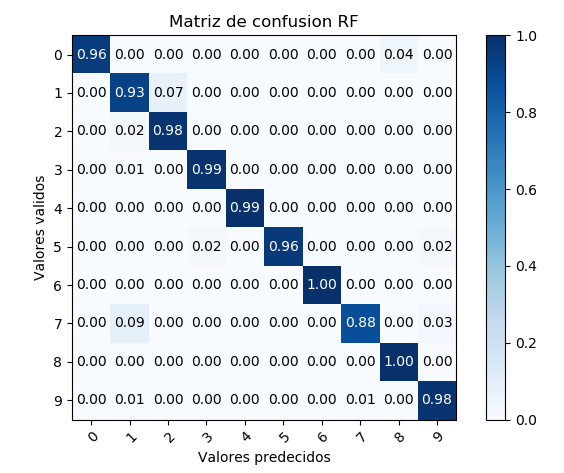
\includegraphics[width=0.7\linewidth]{../imagenesRF/matrizConfusion}
		\caption{}
		\label{fig:Matriz de confusion RF}
	\end{figure}
	
	En este caso se ve que tenemos falla mucho al prediciendo 7 como 1 y también confunde los 1 con 2. Esto nos podría llegar a fallar mas de lo común en el reconocimiento de estos dígitos.
	
	En este caso he querido utilizar una partición de validación en vez de utilizar el método de oob para la validación, por realizarlo de la misma manera que los modelos anteriores.
	
	





\end{document}

